% !TEX root = ../tex/6-4.tex
% 第6章：本文は青、補足は緑
\newcommand{\asmain}{%
    \setbeamercolor{frametitle}{fg=white,bg=main}%
    \setbeamercolor{structure}{fg=main}%
    \setbeamercolor{itemize item}{fg=main}%
    \setbeamercolor{itemize subitem}{fg=main}%
    \setbeamercolor{enumerate item}{fg=main}%
}
\newcommand{\assuppl}{%
    \setbeamercolor{frametitle}{fg=white,bg=examplecol}%
    \setbeamercolor{structure}{fg=examplecol}%
    \setbeamercolor{itemize item}{fg=examplecol}%
    \setbeamercolor{itemize subitem}{fg=examplecol}%
    \setbeamercolor{enumerate item}{fg=examplecol}%
}
% フレームタイトルの「補足」だけを□で囲む
\newcommand{\supplmark}{%
    \setlength{\fboxsep}{1.5pt}%
    \setlength{\fboxrule}{0.7pt}%
    \fbox{\textbf{補足}}%
}
\asmain


%=============================================
\begin{frame}{6.4 Beneath It All: The Fokker--Planck Equation}
    \begin{block}{この節の位置づけ（論文 6.4）}
        変分・スコア・フローの三視点を、\\
        \textbf{連続の式 / Fokker--Planck} という一つの法則の下にまとめる。
    \end{block}
    \begin{itemize}
        \item 三視点は別物ではなく、同じ周辺密度発展を実現する生成子
        \item 違いはパラメータ化と学習目標にあり、密度の拘束は共通
        \item Figure~6.2 が全体像。6.4.1 でフローと Score SDE をつなぐ
    \end{itemize}
\end{frame}
%=============================================
\asmain
\begin{frame}{6.4 の道筋}
    \begin{enumerate}
        \item \textbf{統一の原理}\\
        前向き過程が決めた $\{p_t\}$ を、連続の式 / FP が支配する
        \item \textbf{変分 $\leftrightarrow$ SDE}\\
        離散核の周辺化は、連続時間の FP と整合（4.6 の再掲）
        \item \textbf{フロー $\leftrightarrow$ Score SDE（6.4.1）}\\
        同じ $\{p_t\}$ を、ODE と一群の逆時間 SDE が実現する
        \item \textbf{帰結}\\
        $\gamma(t)$ は軌道の確率性を変え、オラクル周辺は保つ
    \end{enumerate}
\end{frame}
%=============================================
\section{統一の原理}
\asmain
\begin{frame}{三視点は同じ密度発展の別表現}
    \begin{columns}[T,onlytextwidth]
        \begin{column}{0.32\textwidth}
            \begin{block}{変分}
                離散核\\
                $p(x_{t-\Delta t}\mid x_t)$\\
                （Bayes）
            \end{block}
        \end{column}
        \begin{column}{0.32\textwidth}
            \begin{block}{スコア}
                連続 SDE\\
                スコア補正\\
                の逆過程
            \end{block}
        \end{column}
        \begin{column}{0.32\textwidth}
            \begin{block}{フロー}
                決定的 ODE\\
                速度場 $v^{*}$\\
                （PF-ODE）
            \end{block}
        \end{column}
    \end{columns}
    \vfill
    \begin{alertblock}{共通の拘束}
        いずれも、前向き過程が定めた周辺列 $\{p_t\}$ を運ぶ生成子である。\\
        密度レベルでは \textbf{連続の式 / Fokker--Planck} が万能の法則。
    \end{alertblock}
\end{frame}
%=============================================
\asmain
\begin{frame}{前向き過程が「公理」側の経路を決める}
    条件付き摂動核
    \[
        p_t(x_t\mid x_0)
        =
        \mathcal{N}\!\bigl(x_t;\;\alpha_t x_0,\;\sigma_t^{2}I\bigr),
        \qquad
        x_0\sim p_{\mathrm{data}}
    \]
    が周辺経路
    \[
        p_t(x_t)
        =
        \mathbb{E}_{x_0\sim p_{\mathrm{data}}}
        \bigl[p_t(x_t\mid x_0)\bigr]
    \]
    を誘導する（$p_T\approx p_{\mathrm{prior}}$）。
    \begin{exampleblock}{読み方}
        生成側の力学（変分核 / 逆SDE / ODE）は、\\
        この $\{p_t\}$ を\textbf{遡って実現する}ための別表現である。
    \end{exampleblock}
\end{frame}
%=============================================
\asmain
\begin{frame}{連続の式 / Fokker--Planck が言うこと}
    決定的な確率流では連続の式
    \[
        \partial_t p_t(x)
        =
        -\nabla_x\cdot\bigl(v^{*}(x,t)\,p_t(x)\bigr)
    \]
    が密度の時間発展を決める。\\
    拡散がある場合は FP になり、ドリフトと拡散が周辺を運ぶ。
    \begin{itemize}
        \item \textbf{同じ $\{p_t\}$} なら、力学の形が違っても密度拘束は同じ
        \item 軌道の揺らぎ（確率性）と、周辺列の一致は別の話
        \item 学習は「この密度発展を運ぶ場」を当てること
    \end{itemize}
\end{frame}
%=============================================
\asmain
\begin{frame}{Figure 6.2 --- 三視点の統一図}
    \centering
    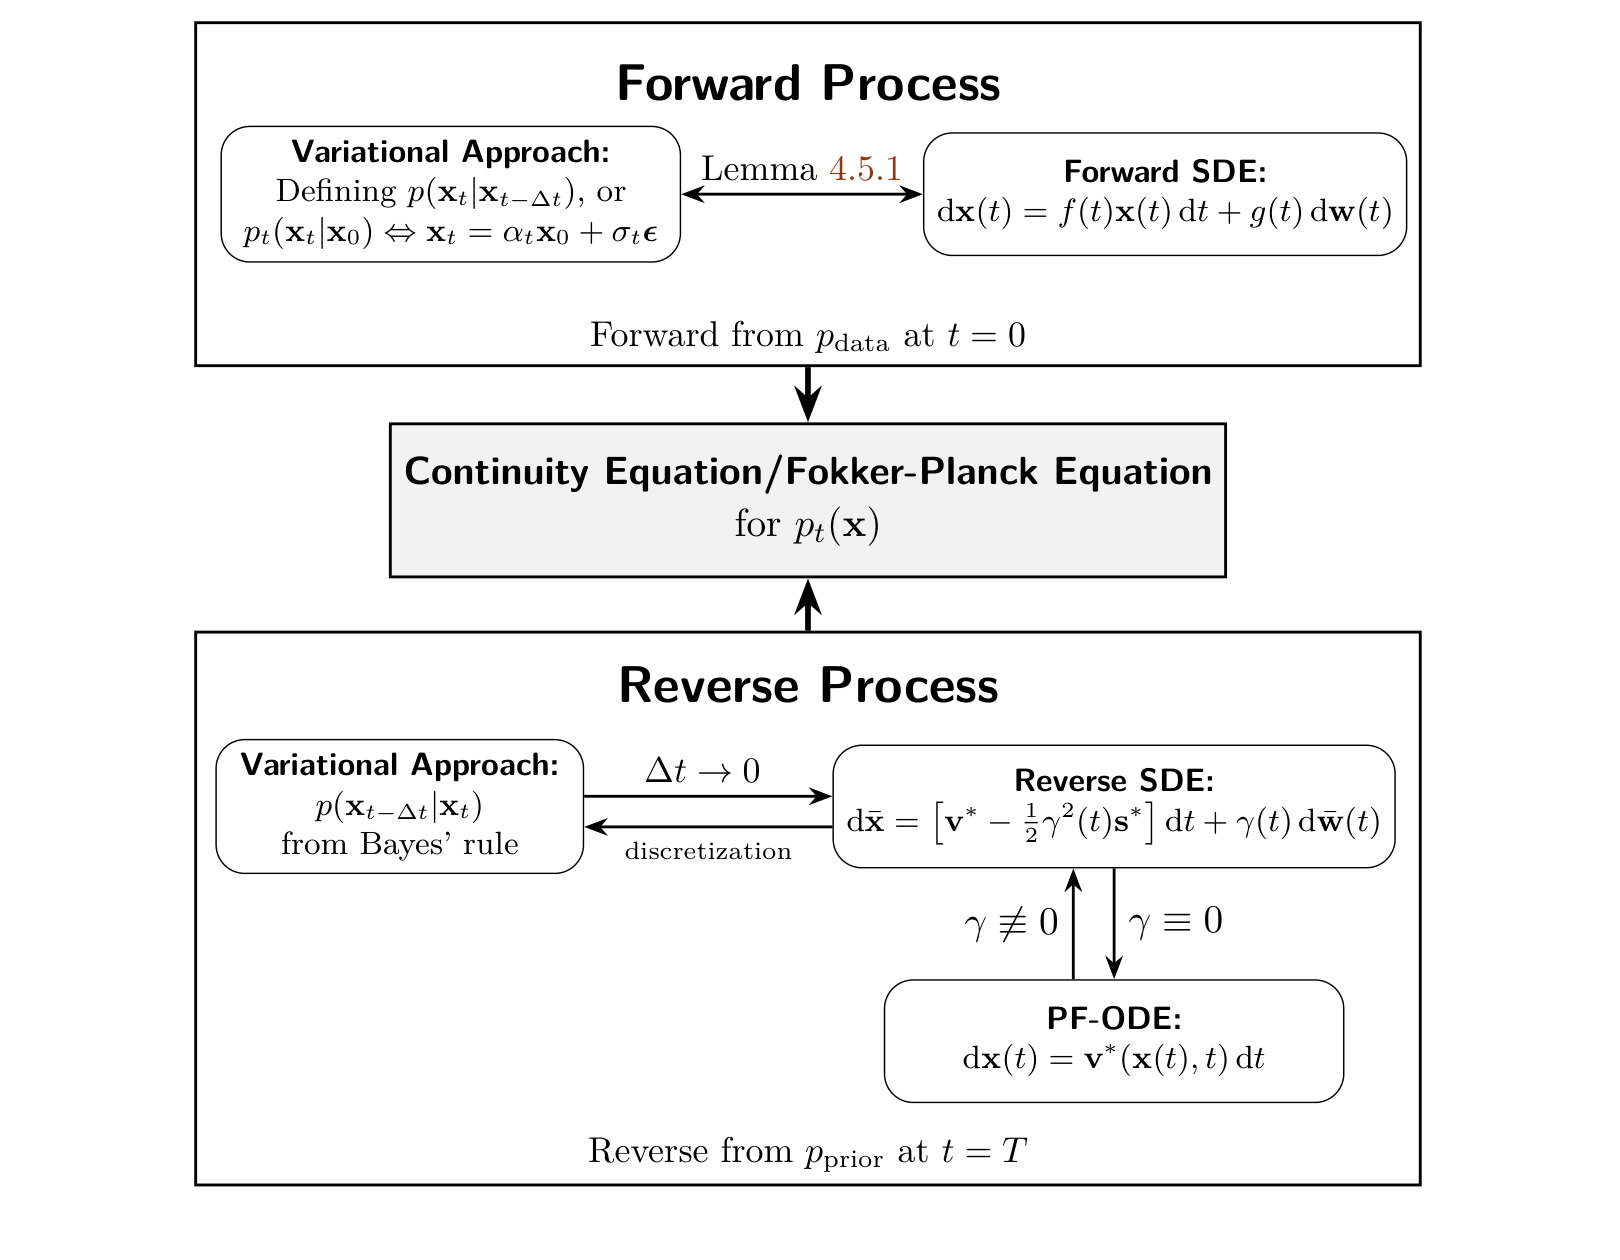
\includegraphics[height=0.72\textheight]{fig-6-2.jpg}
    \vfill
    \footnotesize
    Continuity / FP を中心に、前向きと逆向きの表現がつながる。\\
    Source: Created by the authors.\ （論文 Figure~6.2）
\end{frame}
%=============================================
\asmain
\begin{frame}{Figure 6.2 の読み方}
    \begin{enumerate}
        \item \textbf{Forward}：変分の離散核 $\;\leftrightarrow\;$ 前向き SDE\\
        （Lemma~4.5.1 で接続）
        \item \textbf{中心}：どちらの過程も、同じ $p_t$ の連続の式 / FP に従う
        \item \textbf{Reverse}：Bayes の変分核 $\;\leftrightarrow\;$ 逆時間 SDE\\
        （$\Delta t\to 0$ / 離散化）
        \item \textbf{$\gamma$}：$\gamma\equiv 0$ で PF-ODE、$\gamma\not\equiv 0$ で確率的逆過程
    \end{enumerate}
    \begin{block}{オラクル速度}
        $v^{*}(x,t)=f(t)x-\tfrac12 g^{2}(t)s^{*}(x,t)$、
        $s^{*}:=\nabla_x\log p_t$。
    \end{block}
\end{frame}
%=============================================
\section{変分と SDE の接続}
\asmain
\begin{frame}{変分視点 $\leftrightarrow$ Score SDE（4.6 の要約）}
    第4章 4.6 の議論を、統一図の上側・下側として再掲する。
    \begin{itemize}
        \item 離散の前向き核を細かくすると、前向き SDE の FP に整合
        \item 逆遷移を Bayes で書くと、スコア補正つきの逆過程が出る
        \item よって変分モデルは、連続時間 SDE の\textbf{整合的な離散化}
    \end{itemize}
    \begin{exampleblock}{ここでの要点}
        「離散の変分」と「連続のスコアSDE」は別理論ではなく、\\
        同じ密度発展の表現粒度が違うだけである。
    \end{exampleblock}
\end{frame}
%=============================================
\assuppl
\begin{frame}{\supplmark：離散核と連続力学の対応}
    \centering
    \renewcommand{\arraystretch}{1.35}
    \footnotesize
    \begin{tabular}{lll}
        \textbf{側} & \textbf{変分（離散）} & \textbf{Score SDE（連続）} \\
        \hline
        前向き
        & $p(x_t\mid x_{t-\Delta t})$ / $\alpha_t,\sigma_t$
        & $\mathrm{d}x=f(t)x\,\mathrm{d}t+g(t)\,\mathrm{d}w$
        \\
        逆向き
        & $p(x_{t-\Delta t}\mid x_t)$（Bayes）
        & スコア補正つき逆時間 SDE
        \\
        密度
        & ステップごとの周辺
        & Fokker--Planck の連続発展
        \\
    \end{tabular}
    \normalsize
    \vfill
    周辺の一歩ずつの計算が、連続極限で FP と一致する（4.6）。
\end{frame}
%=============================================
\section{6.4.1 Flow と Score SDE}
\asmain
\begin{frame}{6.4.1：フローと Score SDE の接続}
    \begin{block}{ねらい}
        決定的 ODE（第5章）が定める密度経路を、\\
        一群の確率的逆時間 SDE でも実現できることを示す。
    \end{block}
    \begin{itemize}
        \item ODE と SDE は対立ではなく、\textbf{同じ FP 族}の両端
        \item ブリッジはオラクル速度 $v^{*}$ とスコア $s^{*}$ の関係
        \item 結果として「ODE $\leftrightarrow$ SDE」の連続な家族が得られる
    \end{itemize}
\end{frame}
%=============================================
\asmain
\begin{frame}{設定：ガウス摂動と生成 ODE}
    摂動核 $p_t(x_t\mid x_0)=\mathcal{N}(x_t;\alpha_t x_0,\sigma_t^{2}I)$ の下で、
    密度経路を運ぶ ODE
    \[
        \frac{\mathrm{d}x(t)}{\mathrm{d}t}
        =
        v_t\bigl(x(t)\bigr),
        \qquad
        t\in[0,T]
        \tag{6.4.1}
    \]
    を考える。オラクル速度は
    \[
        v_t(x)
        =
        \mathbb{E}\bigl[\alpha_t' x_0+\sigma_t'\epsilon\mid x\bigr]
    \]
    （式~(5.2.9)；時間向きは拡散モデルの慣習に合わせる）。
    \begin{exampleblock}{生成}
        $x(T)\sim p_{\mathrm{prior}}$ から (6.4.1) を逆向きに積分すると $p_0$ の標本。
    \end{exampleblock}
\end{frame}
%=============================================
\asmain
\begin{frame}{Question 6.4.1}
    \begin{block}{問い}
        事前 $p_{\mathrm{prior}}$ から出発し、\\
        ODE~(6.4.1) と\textbf{同じ周辺密度}を与える SDE はあるか？
    \end{block}
    \begin{itemize}
        \item ODE だけでも高品質な生成は可能
        \item 確率性を足すと、多様性や数値挙動が変わることがある
        \item 答え：同じ $\{p_t\}$ を誘導する\textbf{逆時間 SDE の族}がある
    \end{itemize}
\end{frame}
%=============================================
\asmain
\begin{frame}{Proposition 6.4.1（主張）}
    任意の $\gamma(t)\ge 0$ に対し、逆時間 SDE
    \[
        \resizebox{0.95\textwidth}{!}{$
        \mathrm{d}\bar{x}(t)
        =
        \Bigl[
            v^{*}(\bar{x},t)
            -
            \tfrac12\gamma^{2}(t)\,s^{*}(\bar{x},t)
        \Bigr]
        \mathrm{d}t
        +
        \gamma(t)\,\mathrm{d}\bar{w}(t)
        $}
        \tag{6.4.2}
    \]
    （$t:T\to 0$、$\bar{x}(T)\sim p_T$）は、ODE が定める周辺列 $\{p_t\}$ と一致する。
    \begin{exampleblock}{ポイント}
        $\gamma$ を変えてもオラクルの\textbf{一時刻周辺}は変わらない。
    \end{exampleblock}
\end{frame}
%=============================================
\asmain
\begin{frame}{速度とスコアの関係（6.4.3）}
    \[
        v^{*}(x,t)
        =
        f(t)x
        -
        \tfrac12 g^{2}(t)\,s^{*}(x,t),
        \qquad
        s^{*}(x,t)
        =
        \nabla_x\log p_t(x)
    \]
    スケジュール $(\alpha_t,\sigma_t)$ からは
    \[
        s^{*}(x,t)
        =
        \frac{1}{\sigma_t}\,
        \frac{
            \alpha_t v^{*}(x,t)-\alpha_t' x
        }{
            \alpha_t'\sigma_t-\alpha_t\sigma_t'
       }
    \]
    とも書ける（非退化なスケジュールを仮定）。
    \begin{itemize}
        \item 速度予測 $\leftrightarrow$ スコア予測は代数的に変換可能
        \item 学習後の $v_{\phi^{\times}}$ から経験的逆時間 SDE を組める
    \end{itemize}
\end{frame}
%=============================================
\assuppl
\begin{frame}{\supplmark：証明の骨格（FP の打ち消し）}
    逆時間の Fokker--Planck（元の時間変数 $t$ で書く）は
    \[
        \partial_t p_t
        =
        -\nabla\cdot
        \Bigl(
            \bigl[v^{*}-\tfrac12\gamma^{2}s^{*}\bigr]p_t
        \Bigr)
        -
        \tfrac12\gamma^{2}\Delta p_t.
    \]
    恒等式 $\nabla\cdot(s^{*}p_t)=\Delta p_t$（$s^{*}=\nabla\log p_t$）より、\\
    $\gamma$ 依存の 2 階項が打ち消し、
    \[
        \partial_t p_t
        =
        -\nabla\cdot\bigl(v^{*}p_t\bigr)
    \]
    すなわち PF-ODE の連続の式に戻る。
    \vfill
    \footnotesize
    詳細は Ma et al.\ (2024) Appendix A.2--A.3。
\end{frame}
%=============================================
\asmain
\begin{frame}{$\gamma(t)$ の代表的な選び方}
    オラクル水準では $\gamma(t)$ は任意（周辺は不変）。
    \begin{enumerate}
        \item $\gamma(t)=0$：式~(6.4.1) の PF-ODE に一致
        \item $\gamma(t)=g(t)$：式~(4.1.6) の標準的な逆時間 SDE\\
        （$v^{*}=f x-\tfrac12 g^{2}s^{*}$ を使う）
        \item その他：例として、学習後の KL ギャップを小さくする $\gamma$\\
        （Ma et al., 2024）
    \end{enumerate}
    \begin{alertblock}{実務との違い}
        有限容量ネット・有限ステップ数値解では、$\gamma$ の選びが\\
        多様性や誤差に効きうる。周辺の\textbf{理論的}一致とは別問題。
    \end{alertblock}
\end{frame}
%=============================================
\asmain
\begin{frame}{学習後の使い方}
    \begin{enumerate}
        \item 速度場 $v_{\phi^{\times}}$ を学習する（Flow Matching など）
        \item 式~(6.4.3) でスコア $s_{\phi^{\times}}$ へ変換する
        \item 選んだ $\gamma(t)$ を (6.4.2) に差し込み、\\
        $t=T\to 0$、$x(T)\sim p_{\mathrm{prior}}$ で数値積分する
    \end{enumerate}
    \begin{block}{柔軟性}
        一度 $\{p_t\}$ を前向き過程で定めれば、\\
        PF-ODE から逆時間 SDE まで、\textbf{同じ周辺}を運ぶ族が手に入る。
    \end{block}
\end{frame}
%=============================================
\asmain
\begin{frame}{密度レベルでの結論}
    $\gamma$ 依存のドリフト・拡散は FP 上で打ち消し、共通の法則
    \[
        \partial_t p_t(x)
        =
        -\nabla_x\cdot\bigl(v^{*}(x,t)\,p_t(x)\bigr)
    \]
    に帰着する。
    \begin{itemize}
        \item $\gamma$：個々の軌道の確率性を制御
        \item $v^{*}$：オラクルの一時刻周辺を決める速度
        \item 決定的 PF-ODE と確率的 SDE は、同じ図の両端（Figure~6.2）
    \end{itemize}
\end{frame}
%=============================================
\asmain
\begin{frame}{万能拘束としての FP}
    \begin{columns}[T,onlytextwidth]
        \begin{column}{0.48\textwidth}
            \begin{block}{共通}
                連続の式 / FP\\
                同じ $\{p_t\}$ の発展
            \end{block}
        \end{column}
        \begin{column}{0.48\textwidth}
            \begin{block}{相違}
                パラメータ化\\
                学習目標・離散化
            \end{block}
        \end{column}
    \end{columns}
    \vfill
    \begin{itemize}
        \item 変分：離散遷移を当てる（ELBO / ノイズ予測など）
        \item スコア：$\nabla\log p_t$ を当て、SDE/ODE を組む
        \item フロー：$v_t$ を直接当て、必要なら SDE 族へ変換
    \end{itemize}
\end{frame}
%=============================================
\asmain
\begin{frame}{6.4 のまとめ}
    \begin{itemize}
        \item 三視点は、同じ周辺密度発展を実現する異なる生成子
        \item Continuity / Fokker--Planck が万能の密度拘束（Figure~6.2）
        \item 変分は連続 SDE の整合的離散化として読める
        \item Prop.~6.4.1：任意 $\gamma\ge 0$ の逆時間 SDE が ODE と同じ $\{p_t\}$
        \item $\gamma$ は軌道の確率性を変え、オラクル周辺は保つ
    \end{itemize}
\end{frame}
%=============================================
\asmain
\begin{frame}{次節へ：Closing Remarks}
    統一の核心（FP）まで見たので、第6章全体を閉じる。
    \begin{enumerate}
        \item 条件付け原理と四つの予測型を振り返る
        \item 「同等」の意味を整理し、到達目標を点検する
        \item 第7章（Optimal Transport）への橋を示す
    \end{enumerate}
\end{frame}
